\subsubsection{INFN Trieste} 
\label{sec:INFN-achieved}
\textbf
{Activity in period 
July 2018 - December 2018}
\par
\begin{enumerate}
\item
\textbf{Test beam studies of the single photon detector 
by MPGD technologies with miniaturized 
pad-size in period July 2018 - December 2018}\\
The prototype architecture consists in two 
staggered THGEM layers, the first one also acting 
as photocathode substrate, followed by a resistive MM 
by discrete elements. The detector active surface is 
100$\times$100~mm$^2$. The THGEM geometrical parameters 
are: 400~$\mu$m hole diameter, 800~$\mu$m pitch, 
400~$\mu$m thickness and hole without a rim.
The MM has 128~$\mu$m gap; the 
pad-size is 3$\times$3~mm$^2$ with 
3.5~mm pitch, for a total number of 
32$\times$32 pads (in total 1024 pads). 
The pads are 
grouped in 32$\times$4  modular 
units; each unit is equipped with a 
connector interfacing the signal 
pads to the front-end electronics 
and a second, identical connector, 
providing the biasing voltage to the 
anode pads via protection resistors, 
one per pad, housed in a dedicated 
resistor board. Figure~\ref{fig:espanso-ibrida}
illustrates the detector design.
The prototype has been built
and fully tested in laboratory, as reported 
in July 2019. The main exercise of the this
reporting period concern the test beam studies of
the prototype performed at CERN over a two-week
period between the end of October and the beginning
of November 2018. In this period, our activities have been partially run in main-user mode and partially in parasitic mode.
%%%%%%%%%%%%%%%%%%%%%%%%%%%%%
\begin{figure}
			\begin{center}
		   		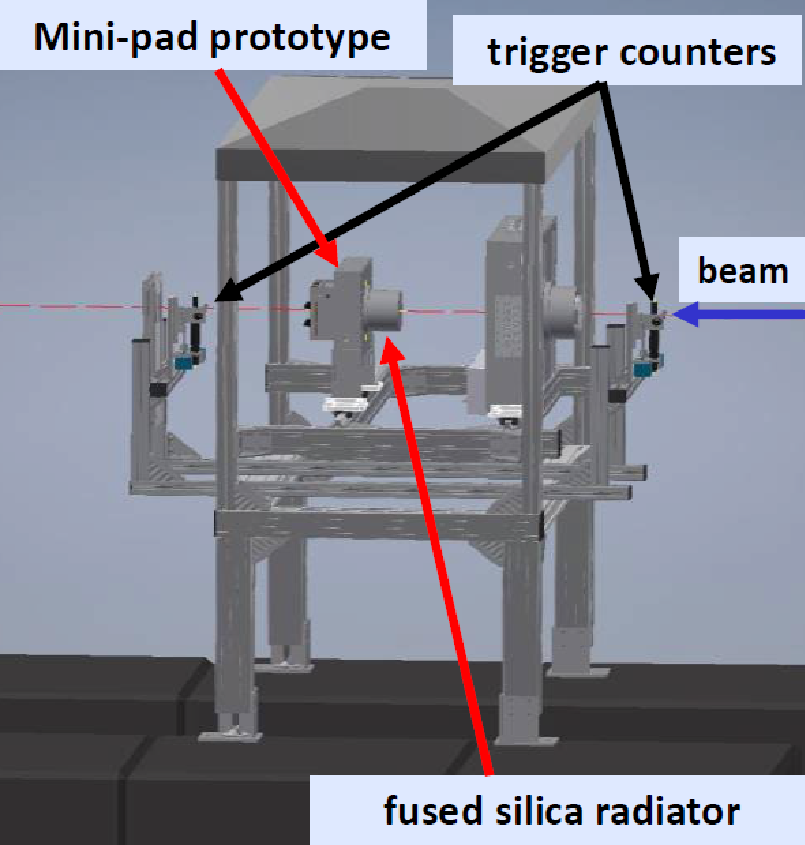
\includegraphics[width=0.7\textwidth
                {INFN_plots/espanso-ibrida}
				\caption{\label{fig:espanso-ibrida}
                Exploded view drawing of the prototype.}
          		\end{center}
			\end{figure}
            %%%%%%%%%%%%%%%%%%%%
The compact test-beam setup for the prototype test was
	prepared, assembled and equipped in Trieste
(Fig.~\ref{fig:set-up_sketch}). It includes:
\begin{itemize} 
\item 
	The mechanical support of the detectors housing also the 
	power supplies, where also top
    and bottom trays to collect methane from leaks,
    if any, are present.
    \item The system of scintillation counters that
    form the trigger: four finger-shaped counters
    are used in coincidence, two placed upstream of
    the prototype and two downstream of it; in both
    couples, the detectors are arrange with
    orthogonal orientation, so to define a cross
    with a small overlap surface of
    3$\times$3~mm$^2$ for the first couple and
    5$\times$5~mm$^2$ for the second one. The
    purpose of this arrangement is to define a 
    select beam particles crossing the detector
    almost perpendicularly and at a well-defined
    location; the finger-shaped counters are
    remotely movable by step motors to facilitate
    the alignment.
    \item The detector with its read-out electronics
    and the power supply for HV and LV.
    \item A fused silica radiator is mounted onto
    the prototype; it has cylindrical symmetry
    and a dedicated design: the majority of the Cherenkov photons
    generated by minimum ionizing particles with trajectories quasi-parallel to its axis populate a ring
    surface of the detector
    (Figs.~\ref{fig:radiator}, \ref{fig:hybrid&radiator}). A shutter is situated between the radiator and the photocathode and it is remotely controlled via a piezoelectric actuator.
    \item The read-out system is based on the SRS/APV25 system~\cite{1748-0221-8-03-C03015} developed within the RD51 collaboration. The 1024 pads are read-out by eight APV25 chips, 128 channel each. The chip control and the DAQ is ensured by the novel DAQ Raven system,  entirely
LabView based, developed with the current activity in order  to enlarge the acquisition band width and reported about in January 2018. Dedicated interface boards have been designed and realized to interface the detector connectors and the SRS/APV25 FE boards.
\end{itemize}
%%%%%%%%%%%%%%%%%%%%%%%%%%%%%%%
\begin{figure}
\begin{center}
%\includegraphics[width=0.6\textwidth]{INFN_plots/set-up_sketch}
\caption{\label{fig:set-up_sketch}
Picture of the setup for the test beam, during assembly in Trieste.
}
\end{center}
\end{figure}
%%%%%%%%%%%%%%%%%%%%%%%%%%%%%%%%%%%%%%%%%%%%%%%%%%%%%%%%%
\begin{figure}
			\begin{center}
     %       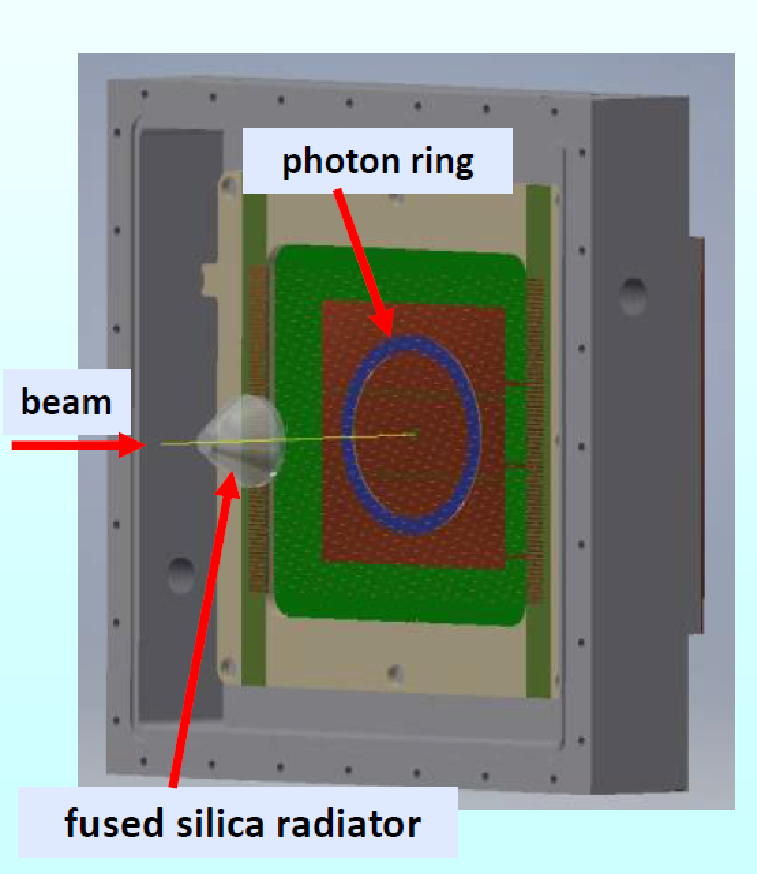
\includegraphics[width=0.7\textwidth{INFN_plots/radiator}
\caption{\label{fig:radiator}
Cross-section of the fused silica radiator with cylindrical symmetry. The blue lines are examples of Cherenkov photon trajectories; a good fraction of them intercept the photocathode surface (the vertical black line in the drawing) in a ring region, even if part of the photons hit the photocathode in different areas. The majority of the photons generated in the radiator are trapped inside the radiator itself due to total reflection; there are no examples of these trajectories in the drawing.
}
			\end{center}
\end{figure}
%%%%%%%%%%%%%%%%%%%%%%%%%%%%%%%
%%%%%%%%%%%%%%%%%%%%%%%%%%%
\begin{figure}
			\begin{center}
%\includegraphics[width=0.6\textwidth]{INFN_plots/hybrid&radiator}
\caption{\label{fig:hybrid&radiator}
Skematic drawing illustrating the formation of the ring image in the photon detector using the fused silica radiator. 
}
			\end center
\end{figure}
%%%%%%%%%%%%%%%%%%%%%%%%%%%%%%%
The last phase of the detector assembly consists in inserting in the detector the THGEM coated with the CsI film, that must not be expose to air in order to preserve its quantum efficiency. This implies that the final assembly is performed in a glove-box (Fig.~\ref{fig:assembly-in_glovebox}).  At this time also the fused silica radiator is added. A picture of the prototype fully equipped and installed at the test-beam is shown in Fig.~\ref{fig:mini-pad_at_test-beam}.                 %%%%%%%%%%%%%%%%%%%%%%%%%
\begin{figure}
			\begin{center}
			%	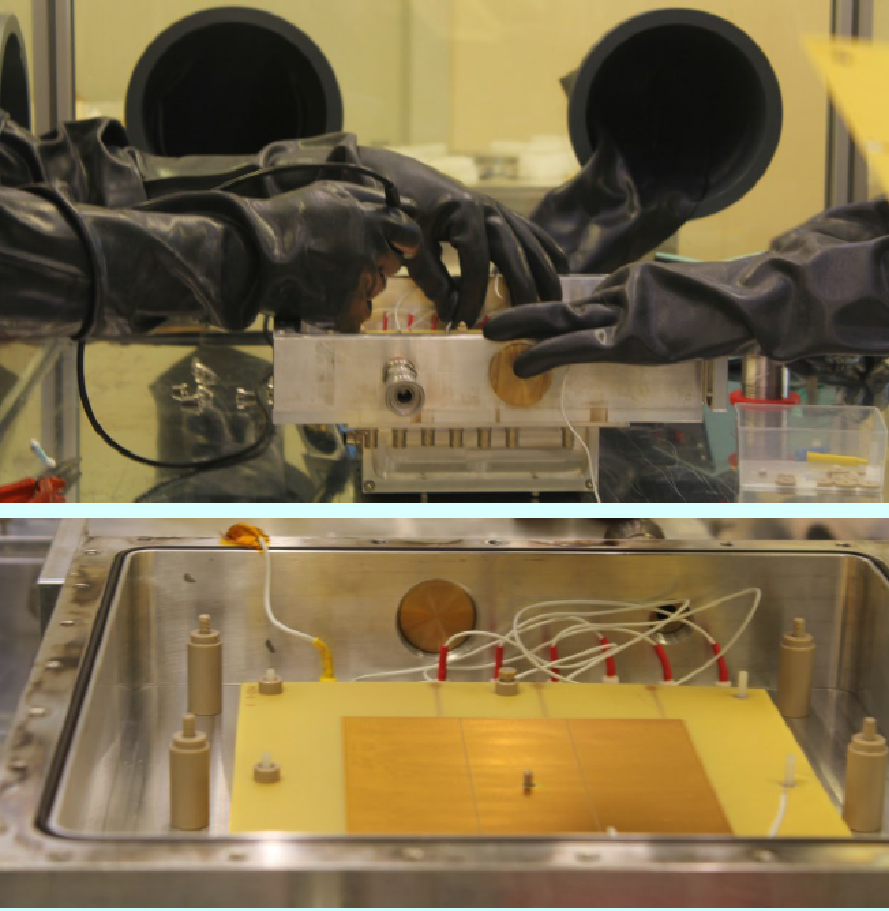
\includegraphics[width=0.6\textwidth]			
                {INFN_plots/assembly-in_glovebox}
				\caption{\label{fig:assembly-in_glovebox}
                	Pictures illustrating the final phase of the 
       						 prototype
                	assembly, which is performed in a glove-box.
               	 }
			\end{center}
            \end{figure}%%%%%%%%%%%%%%%%%%%%%%%%
\begin{figure}
			\begin{center}
			%	\includegraphics[width=0.6\textwidth
                			{INFN_plots/mini-pad_at_test-beam}
				\caption{\label{fig:mini-pad_at_test-beam}
                Picture of the fully-equipped prototype 
                		installed at the
                test-beam.
                }
			\end{center}
            \end{figure} 
            %%%%%%%%%%%%%%%%%%  
       Data have been collected using two different gas mixture, 
       namely (a) Ar:CH$_4$~=~50:50 and (b) pure methane. Data have 
       been collected with different voltage settings in order 
       to determine the 
       optimal operation conditions. The data analysis has just 
       started and in the following we provide some preliminary 
       information obtained from the data collected with gas 
       mixture (a). It is relevant to underline that, aiming at single 
       photoelectron detection, we have to deal with an exponential 
       amplitude spectrum, where the majority of the population is 
       at small amplitudes. Therefore, we have to apply small 
       threshold-values and the good control of the noise treatment  
       is important. At present, we could not yet implement the 
       subtraction of the common-mode noise and, therefore, the 
       following preliminary plots are still affected by 
       non-negligible noise contributions. At present, the software threshold applied to the amplitude is at the 4.5$\times$ the noise r.m.s. .
       The time development of a typical signal is shown in Fig.~\ref{fig:APV_signal}:  27 consecutive measurements of the signal amplitude measured in all the 128 channels of an APV chip, 25~ns time-distance,  are shown. The image was obtained on-line using one of the feature of the RAVEN DAQ system.  In the following, the time associated to the heighest amplitude measurement is used: the time distribution respect to the trigger time is shown in Fig.~\ref{fig:timing_plot-1}. %\par
       The 2-D histogram of the hits for a sample of events collected with the shutter between the radiator and the photocathode open is shown in Fig.~\ref{fig:Iris_open_Ar_CH4}. A ring is claerly visible as well as, at the center of the ring, the hits due to the minimum ionizing particles crossing the detector. In a corresponding histogram for data collected with the shutter closed (Fig.~\ref{fig:Iris_closed_Ar_CH4}) the ring is no longer visible, while the particle signal is still present. Subtracting the second histogram from the first one applying proper normalization with the number of events, the particle signal disappears, while the ring is claerly visible (Fig.~\ref{fig:subtraction_open_closed}. %\par
     A preliminary algorithm performing hit clusterization is applied to the hits in the ring area and the distribution of the cluster amplitude is used to extract information about the detector gain, as shown in Fig.~\ref{fig: gain_fit-2}: the resulting gain has the remarkable value of 50k. 
     %\par
     The analysis of the test-beam data is in a very initial phase and has to be continued and improved in the coming months. nevertheless, the first indications are very positive: the prototype has been successfully operated at large gain.
\item
Initial studies to understand the 
compatibility of an \textbf{innovative photocathode 
based on NanoDiamond (ND) particles} with the 
operation in gaseous detectors and, in 
particular, in MPGD-based photon detectors\\
The results of the characterization of the first THGEMs 
coated with ND powder have been reported in July 2018. 
An aspect was surprising and puzzling: the THGEMs with
non-hydrogenated ND powder coating exhibit 
higher gain for a given biasing voltage respect 
to the gain measured for 
the same THGEM before applying the coating.
The characterization measurements have been repeated, confirming 
the result, while a possible explanation is emerging.
The coating layer is resistive and it covers both the 
metallized part and insulating part of the THGEM. 
Therefore, its presence is most likely
preventing the charging up of the insulating surfaces. 
It is expected that the THGEM multiplication is 
higher when there is no charging up. The explanation 
has to be supported by further measurements. 
%\par
In parallel, actions towards material procurement 
are taking place, 
both concerning new ND powder samples and small-size THGEMs.
\end{enumerate}
%\par 
Concerning the \textbf{dissemination of the results}, 
the initial results concerning the performance of the photon
detector prototype with miniaturized pads have been present at 
\textbf{the 
14$^{th}$ Pisa Meeting on Advanced Detectors},
La Biodola, Isola d'Elba (Italy), 27 May - 02 June 2018,
\cite{AGARWALA2018-2} and at \textbf{the 
10th International Workshop on Ring Imaging Cherenkov Detectors}, 
Moscow (Russia) 29 July – 4 August 2018.
The first studies concerning the coupling of ND photocathodes and MPGDs have been presented at \textbf{the 
10th International Workshop on Ring Imaging Cherenkov Detectors}, 
Moscow (Russia) 29 July – 4 August 2018\cite{Agarwala:2018qdm}.
%\par
Concerning the 
\textbf{milestones for 2018}:
\begin{itemize}
\item
\textbf{September 2018: The completion of the laboratory 
characterization 
of the photon detector with miniaturized pad-size.}\\
The exercise has been completed and the milestone is
successfully matched.
\item
\textbf{September 2018: 
The performance of the tests to establish the 
compatibility of the ND photocathodes with the
operation of MPGD-based photon detectors.}\\
The tests have been performed and, therefore, the
milestone is partially matched. Nevertheless, there is
not yet a solid answer to the question related to the
compatibility:  
the totally
unexpected results demand 
for further investigation in 2019.
\end{itemize}